%%%%%%%%%%%%%%%%%%%%%%%%%%%%%%%%%%%%%%%%%%%%%%%%%%%%%%%%%%%%%%%%%%%%%%%%%%%%%%%%%%
%%% Navigation Control
%%%
%%%
%%%%%%%%%%%%%%%%%%%%%%%%%%%%%%%%%%%%%%%%%%%%%%%%%%%%%%%%%%%%%%%%%%%%%%%%%%%%%%%%%%
\chapter{Perception and Navigation}
\label{ch::navigation}


	\section{Flatland navigation and goal (feature) tracking}
	
		The BlueFoot robot is operated using potential field-based control-schemes for obstacle avoidance and camera-based goal-tracking over flatland. Platform navigation is administered by two main command parameters, $v^{r}$ and $\omega^{r}$, which represent forward and turning rate of the platform with respect to the robot's trunk frame $O_{b}$. During navigation, the pitch of the trunk, $\theta_{b,x}$ is also controlled via its respective reference signal, $\theta_{b,x}^{r}$. Control over trunk pose allows for additional articulation of the LIDAR and camera sensors mounted to BlueFoot's head (trunk). 

		BlueFoot's base navigation and obstacle avoidance algorithm involves a potential fields-based approach which fuses LIDAR data and features from processed camera images. This algorithm is essentially used as a ``wandering" mechanism which would normally be employed as a first-level navigation measure in an unknown environment when no information (\EG map data) is known by the robot \emph{apriori}. Camera features are used in conjunction with LIDAR scans for the purpose of assigning trackable targets, which are particularly useful for the purpose of avoid local minima faced with navigating via a potential-fields approach alone. These targets are used to \emph{attract} the robot platform towards the target location. Notably, the total navigation approach to be described uses only 2D LIDAR data (does not take into account features of terrain) and is thus most fit for navigation over flatland.

		\subsection{LIDAR-based Potential-Fields Algorithm}
			The LIDAR-base portion of this algorithm takes sequential, planar LIDAR scans as an input and generates a set of navigation outputs, $\vec{u}^{r}_{L} \in \Re^{3}$, which represents a direction of travel relative to the world frame, $O_{0}$, and $p_{L}$, which represents a total positive potential . Each point from a LIDAR scan is mapped to a corresponding scalar \emph{potential} which is used to influence the direction of the newly generated command. Given a LIDAR scan $S$ with 2D scan points, $x_{i}^{L}\in\emph{S}^{L}$, relative to the LIDARs local coordinate frame $O_{L}$, an output command vector is generated using a potential function $\{ f(x) : \Re^{3}\rightarrow \Re^{1} \}$, and a biasing function, $\{ g(x,\psi) : \Re^{3}\rightarrow \Re^{1} \}$, as follows:
				\begin{eqnarray}
				x_{i}  &=& P_{ \vec{z} } \wrap{ H_{b}^{0} H_{L}^{b} \Gamma_{L} x_{i}^{L} } \nonumber\\
				\bar{x}_{b,i} &=&  x_{i}-p_{b} \nonumber \\
				\vec{u}^{r}_{L} &=&  { \sum_{x_{i} \in \emph{S}} g( \bar{x}_{b,i},\psi)  f( \bar{x}_{b,i} ) \frac{\bar{x}_{b,i}}{\norm{\bar{x}_{b,i}}} } \nonumber \\
				p_{L} & = & \alpha_{p}\sum_{x_{i} \in \emph{S}} g( \bar{x}_{b,i},\psi)  f( \bar{x}_{b,i} ) U\wrap{f( \bar{x}_{b,i} )}
				\end{eqnarray}
			where $H_{b}^{0}$ defines a homogeneous transformation between $O_{0}$ and $O_{b}$; $H_{L}^{b}$ defines a homogeneous transformation which relates the LIDAR sensors pose to the frame $O_{b}$; $\emph{S}\subset \Re^{3}$ is the set of newly transformed points, $x_{i} \in \emph{S}$ which respect the current LIDAR scan in the world coordinate system; $U(*)$ is the standard unit-step function;  $\alpha_{p}$ is a scalar tuning parameter; and 
				\begin{equation*}
					\Gamma_{L} = \sbrack{ I_{2\times2}, 0_{2\times1} }^{T}.
				\end{equation*}
			Since we are assuming navigation over flat ground, the operator $P_{ \vec{z} }\wrap{*}$ is used to project each transformed LIDAR scan-point onto the plane defined by the unit vector pointing in the direction of the $z$-axis of the frame $O_{0}$.

			The piecewise potential function, defined in \ref{eq::min_dis_potential_function}, is used in BlueFoot's navigation scheme is designed to ``repel" the platform from objects which are at some minimum distance, $d_{min}$ from the trunk, and attracted toward objects that are further away. The form of this potential function is inspired by several potential function candidates for attractive/repulsive force-field functions presented in \cite{ArambulaCosio2004}. The function \ref{eq::min_dis_potential_function} tends to draw the robot towards long apertures, such as corridors or openings, and away from close-by obstructions. It is written as follows:
				\begin{eqnarray}
					\Delta d &\equiv& \norm{x}-d_{min} \nonumber \\
					f(x) &=& 
					\begin{cases}	
					 	 -\lambda_{c,1} \wrap{\Delta d}^{2} &  \text{if } \Delta d < 0 \\
						\wrap{\Delta d} \wrap{ 1  - e^{ -  \lambda_{c,2} { \wrap{\Delta d} }^{2} } } 	&  \text{else}
					\end{cases}
				\label{eq::min_dis_potential_function}
				\end{eqnarray}
			where $\lambda_{c,1}>0$ and $\lambda_{c,2}>0$ are tuning parameters used to specify the output range and sensitivity of the potential function output with respect to $\Delta d$, respectively. It can be observed that this potential function exhibits $f(x)<0$ when $\norm{x} < d_{min}$ and vice-verse, thus achieves the desired attractive and repulsive characteristics. Namely, this potential function favors points which are generally much further away from the robot, and applies \emph{strong} repulsive forces only when obstacles come within a close range with the platform. These characteristics offer a higher propensity for exploration when the area being navigated is very spacious with few obstacles in view (but at mid range), while encouraging \emph{tight} navigation away from potential obstacles. 

			The biasing function $g(x,\psi)$ is used to weight the effect of individual points from a single scan on the final output, with respect to thier relative angular position. The biasing function is parametrized with an angular-window parameter $\psi>0$. A simple masking-type biasing function is used in BlueFoot's navigation function, which is formally defined as follows:
				\begin{equation}
					g(x,\psi) = 
					\begin{cases}
					1	& \tan^{-1}\wrap{ \frac{x_{2}}{x_{1}} } < \psi \\
					0 	& \text{otherwise}.
					\end{cases}
				\end{equation}
			where $x_{1}$ and $x_{2}$ are the first and second elements of the vector argument $x\in\Re^{3}$. This function is used to give priority points which exists in front for the robot and fall within an angular window $\psi$. Considering only frontward points serves to reduce the potential for getting stuck in local minima, namely when the robot moves into an area where it faces equal potential from all sides. A visualization of  the composite potential field, $f(x)g(x,\psi)$, with $\psi=\pi/2$ is shown in Figure \ref{fig::potential_field} for a $2$-by-$2$ meter area about the robot.
				\begin{figure}[t!]
					\centering
					\fbox{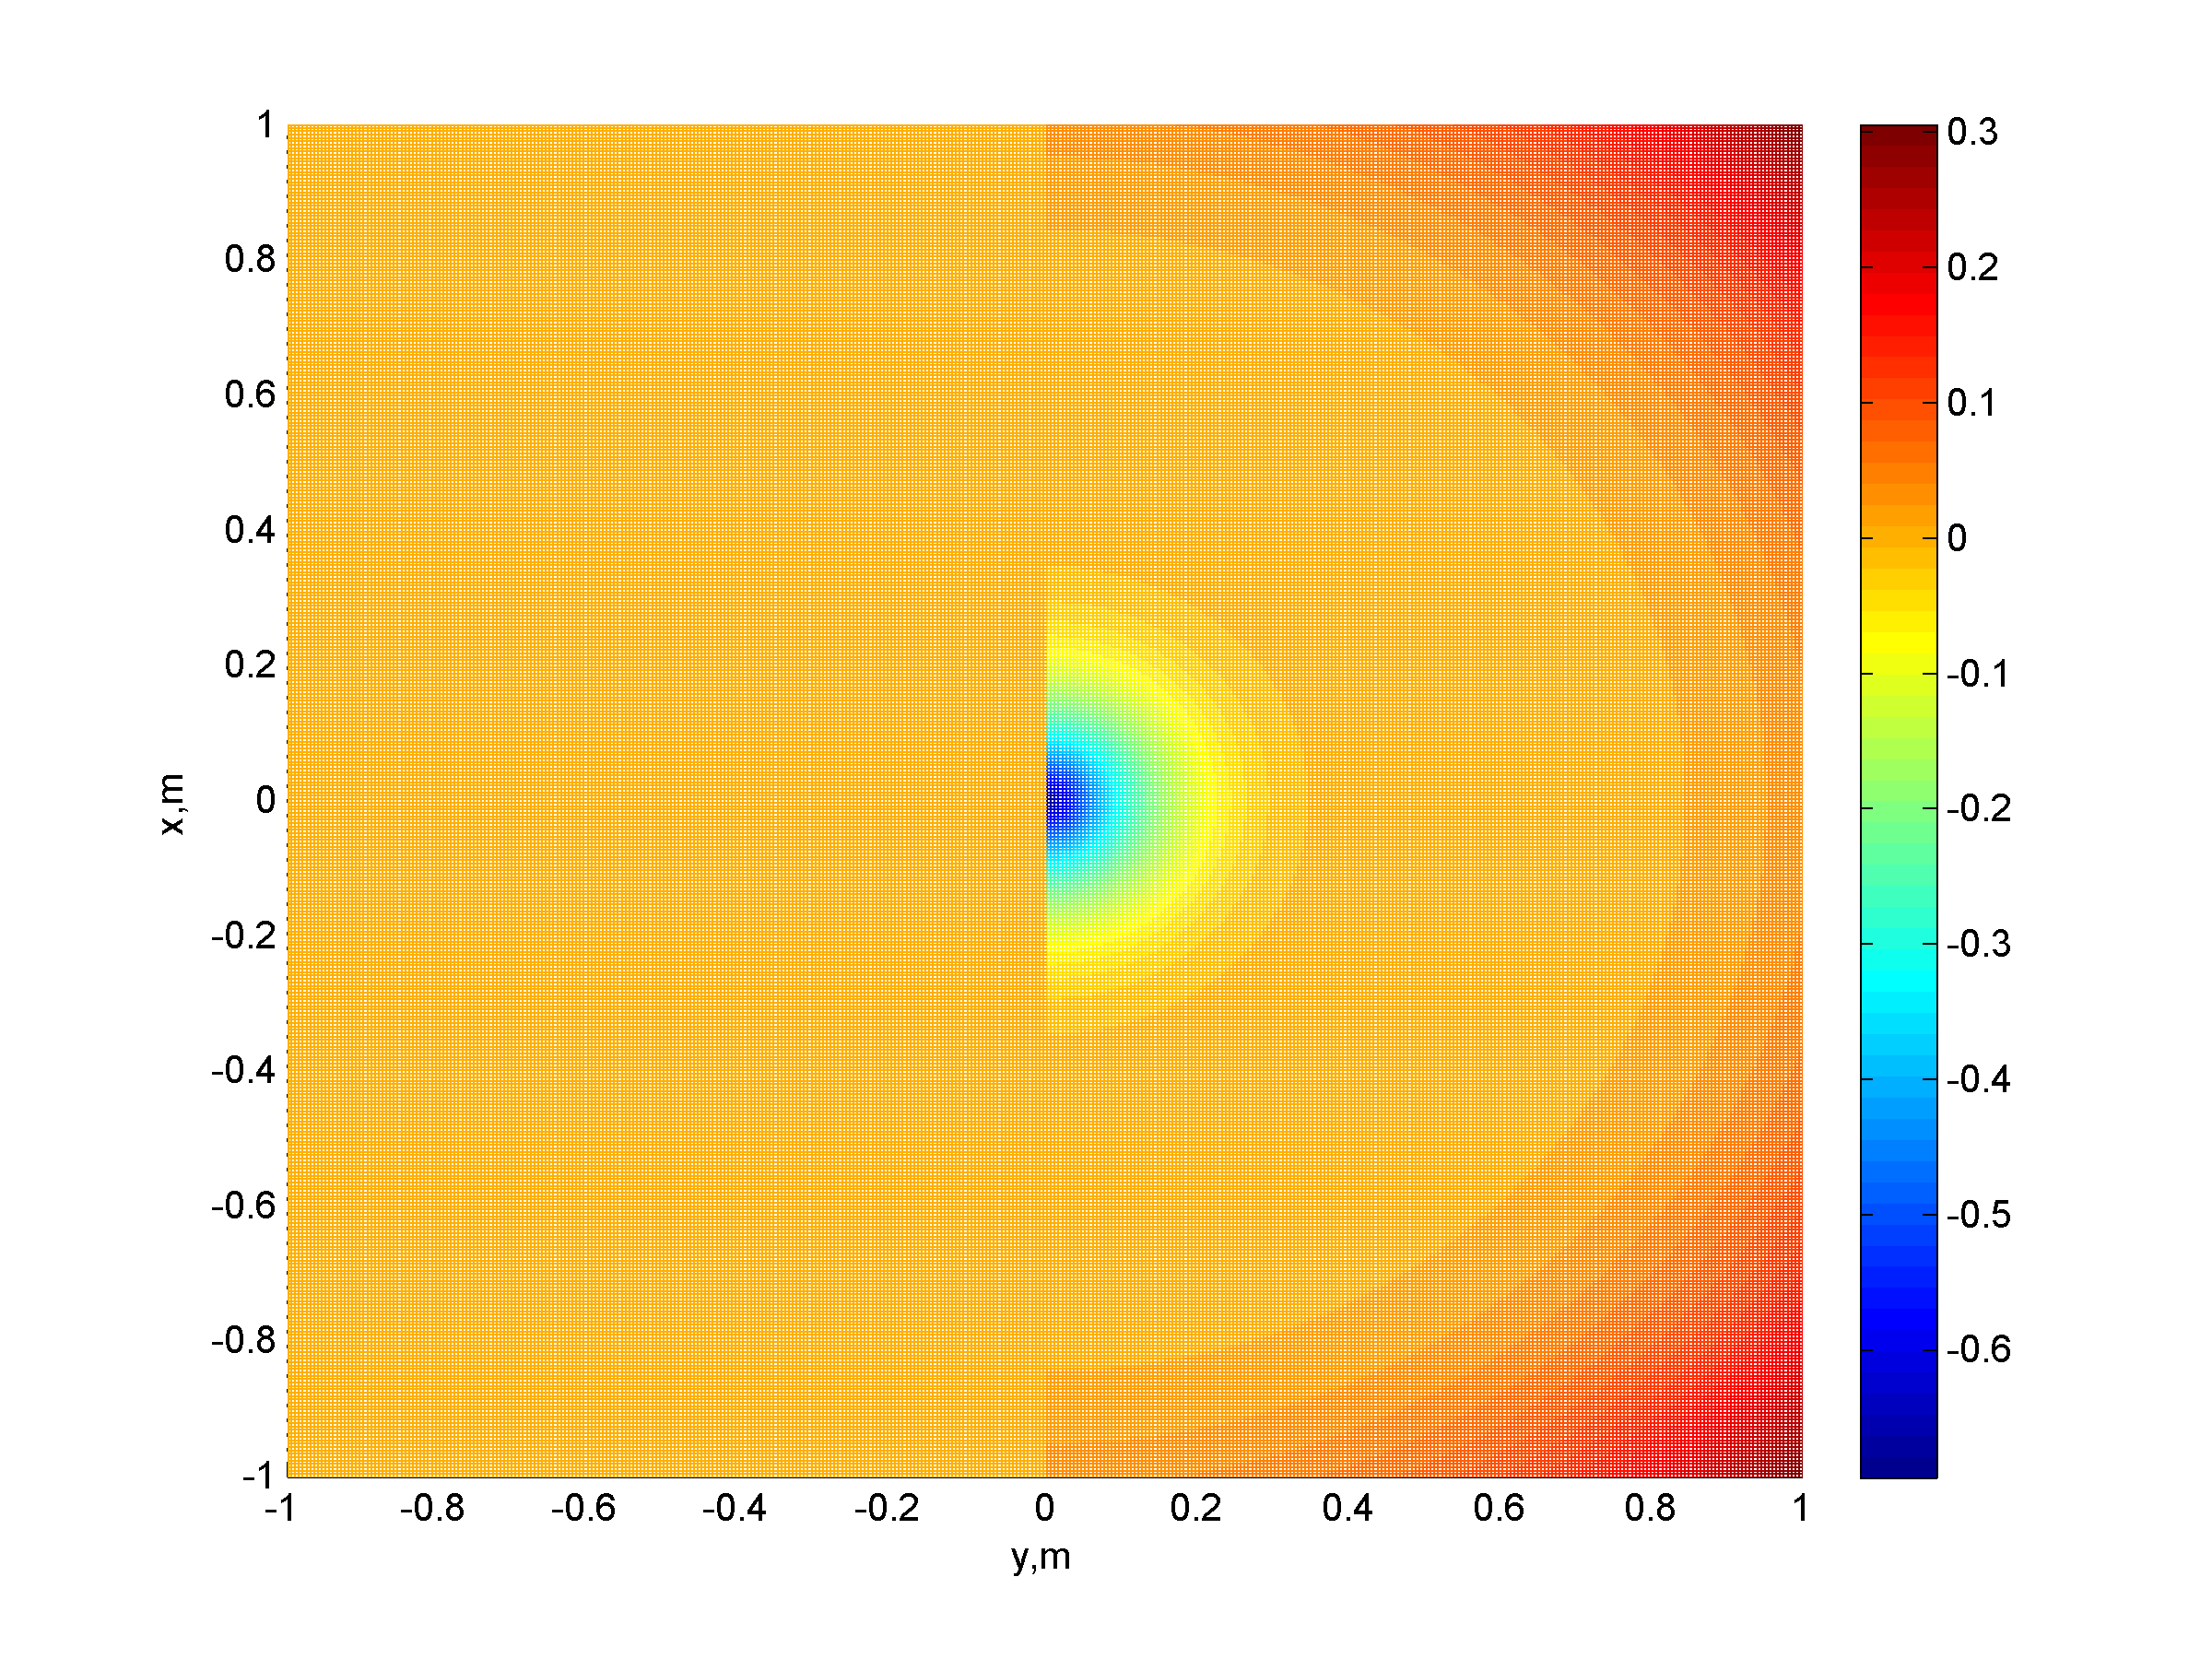
\includegraphics[width=\textwidth]{potential_function.png}}
					\caption{Composite potential field, $f(x)g(x,\psi)$ with $d_{min}=0.4m$.}
					\label{fig::potential_field}
				\end{figure}
			%In the event that the robot does get stuck in a potential minima, a ``stuck" detection algorithm has been implemented. As the name suggests, this algorithm first detects if the robot is stuck in a local minima of the potential field based on a window of command histories.

			Finally, outputs of the potential field algorithm are transformed into forward and turning rate commands, ${v}_{L}^{r}$ and $\omega_{L}^{r}$, respectively, by the following proportional control scheme:
				\begin{eqnarray}
					\theta_{L}^{r} 			&=& \tan^{-1}\wrap{ \frac{(\vec{u}^{r}_{L})_{2} }{(\vec{u}^{r}_{L})_{1}} } \nonumber\\
					\dot{v}_{L}^{r} 		&=& \beta_{v} \wrap{ p_{L} + v_{L,min}^{r} - v_{L}^{r} } \nonumber \\
					\dot{\omega}_{L}^{r} 	&=& \beta_{\omega} \wrap{ \wrap{ \frac{ \omega_{L}^{r,max} }{\pi} } \wrap{  \theta_{L}^{r} - \theta_{b,z} } - \omega_{L}^{r} }
				\end{eqnarray}
			where $\beta_{v}$ and $\beta_{\omega}$ are proportional-gain tuning parameters; $v_{L,min}^{r}>0$ is a small, minimum velocity used to prevent the robot from getting stuck in local minima; and $\theta_{b,z}$ is robot's yaw in $O_{0}$. The parameters $\beta_{v}$ and $\beta_{\omega}$ can be viewed as ``update-inertias," as they directly effect the influence of the effect of instantaneous commands on the forward velocity and turning rate of the robot. Furthermore, these gains can be used to low-pass navigation updates to remove jitter cause by command outliers generated from degenerate sensor readings.


		\subsection{Results of LIDAR-based potential field navigation from simulation}

				\begin{figure}[h!]
					\centering
					\fbox{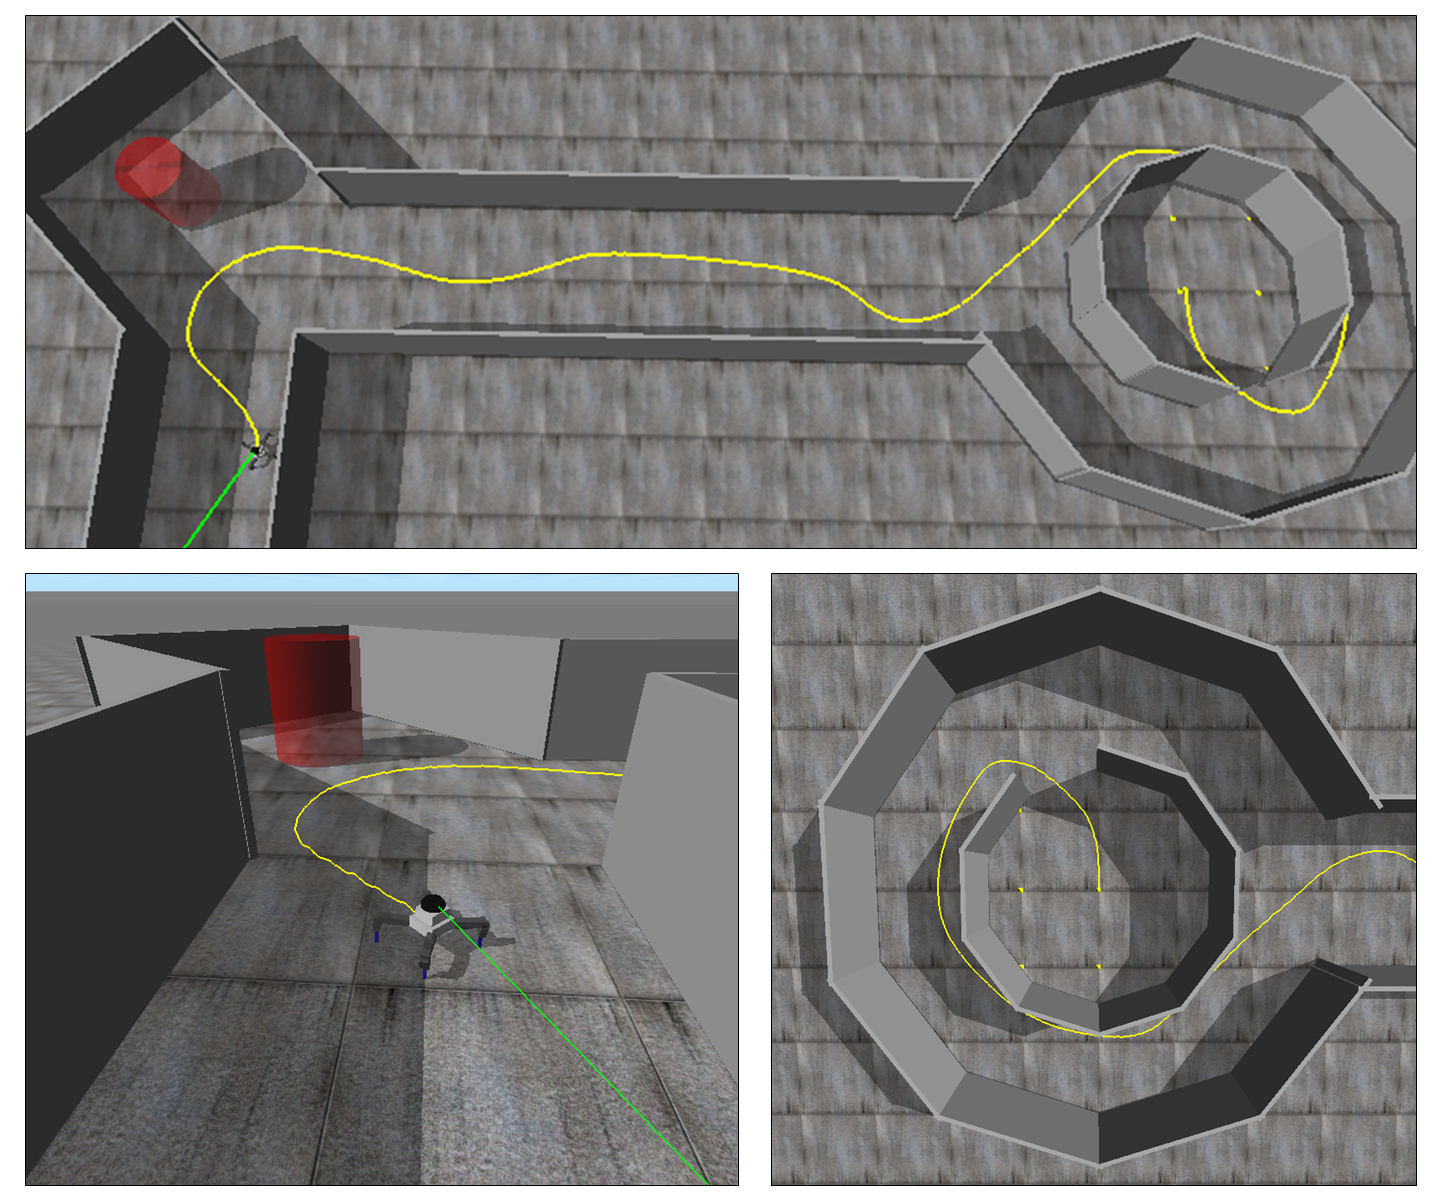
\includegraphics[width=\textwidth]{potential_field_full.png}}
					\caption{Path (shown in yellow) taken by robot through a simulated set of rooms and halls using the LIDAR-based potential fields navigation scheme.}
					\label{fig::potential_field_results}
				\end{figure}
				\begin{figure}[h!]
					\centering
					\fbox{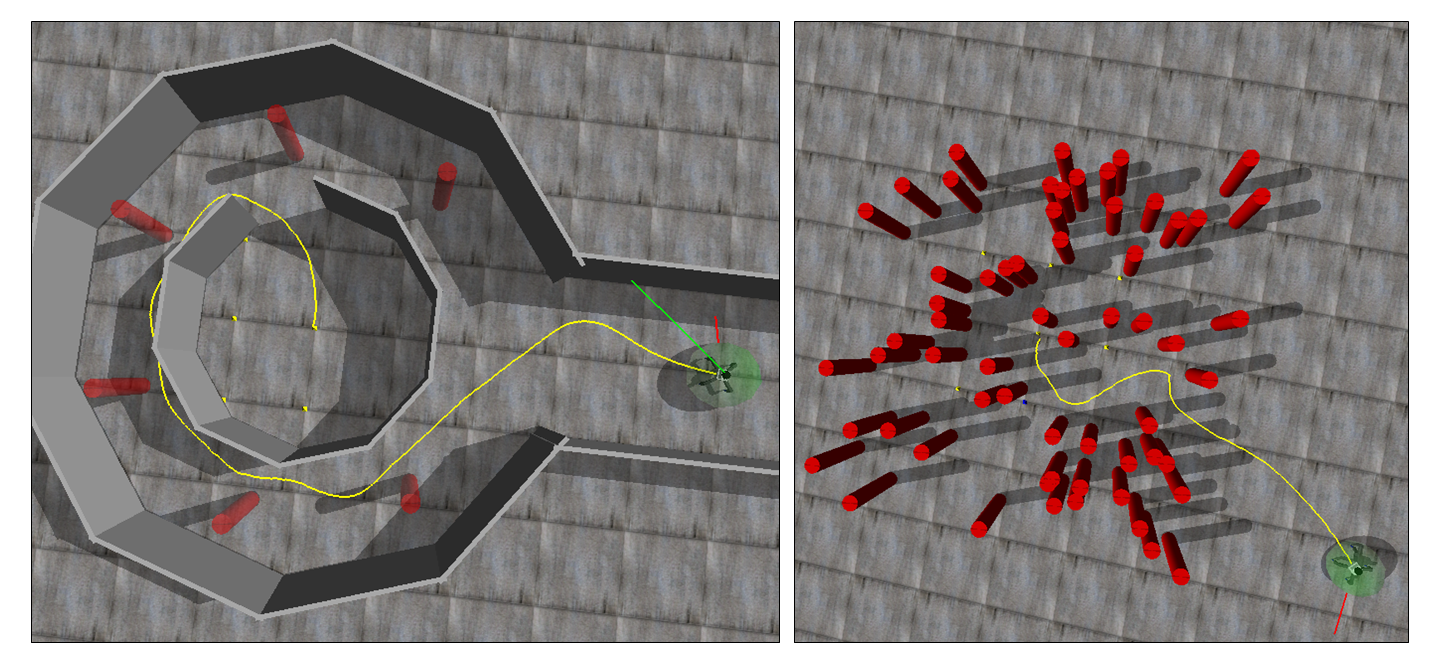
\includegraphics[width=\textwidth]{potential_field_full_obstacles.png}}
					\caption{Path (shown in yellow) taken by robot through a simulated set of rooms and obstacles.}
					\label{fig::potential_field_results_obstacles}
				\end{figure}
		
			Figure \ref{fig::potential_field_results} shows the patch resulting from a simulated trial in which the BlueFoot robot robot autonmously wandered trhough an environment, consisting of a room and several long corridors, using the previously described potential fields formulatons. A plot of the robot's trajectory shows that the robot was able to successfully navigate the region while avoiding collisions with the surrounding walls. Notably, the robot naturally avoided smaller outcove regions, which were filled with obstacles, because these regions had low relative potential. This is becuase of thier relative depth with respect to the robot's position. 

			A second set of results is shown in Figure \ref{fig::potential_field_results_obstacles} shows the robot's performance in enviroments additional obstacles.

		\subsection{Incorporation of Camera-based Feature-Tracking}
		
			Camera-based goal tracking is used in conjunction with the aforementioned potential fields navigation scheme to move the platform through an environment while seeking or tracking a particular target. In this case, targets take the the form of features extracted from processed camera data. The robot is guided towards these features using a visual-serving approach. 

			Trackable camera features can be generated in a variety of ways. For the purpose of BlueFoot's navigation, objects with distinct shapes or color have been chosen for tracking so that shape and blob detection algorithms can be employed to detect their positions relative to BlueFoot's camera view range. Namely, Bluefoot's image processing routines make use of the Hough Transform-based shape detection and standard color-blob detection algorithms available from the Open Computer Vision (OpenCV) libraries \cite{opencv_library}. Once detected, center-positions of each feature, represented with respect to the 2D camera-viewing frame, are mapped into forward rate and turning commands to control the robot towards the relative location of the feature. These camera-based commands are then mixed with the outputs of the potential-fields controller as a weighted sum to form a hybrid navigation control law.

			In this visual-servoing approach, features are used to control the robot in a way that is agnostic of the type of feature being tracked. Namely, this approach relies on the relative position of the center of each features, represented as a pixel-position, $p_{Im} = [u,v]^{T} \in Z^{2}$ in the 2D image frame, $O_{Im}$, and a relative size, $r$, measured in pixels. In the case of circular features, for example, $r$ is represent the radius of the detected circle. For color-blob features, $r$ represents the radius of a circle which fully inscribes the colored object.

			For the purpose of target tracking, it is desired that the robot's forward speed be controlled such that is proportional to $r$. Namely, it is desired that the robot stop when it becomes close to the target object, and move faster when the feature is in sight but the robot is further away. The position of the feature's center is used to control the robot's turning rate, as well as the commanded pitch of the robot's trunk, $\theta_{b,x}^{r}$. Trunk articulation important during feature tracking routing as it aids in keeping the tracked-target objects centered in the image frame. Provided that the target is moving slower than the what the system can achieve, this will ensure the target remains in sight at all times.

			A separate set of navigation commands, $v_{C}^{r}$ and $\omega_{C}^{r}$; and an additional body-pitching command, $\theta_{b,x}^{r}$,  are generated from an extracted feature location, $p_{Im} = [u,v]^{T}$ as follows: 
				\begin{eqnarray}
					v_{C}^{r} 			& = & v_{C}^{r,max} \wrap{ 1 - e^{ -c_{r} \wrap{ r-r_{min} }^{2} } } 	\nonumber 	\\
					\omega_{C}^{r} 	& = & \omega_{C}^{r,max} \wrap{\frac{ w_{Im} - 2 u  }{ w_{Im} } }		\nonumber 	\\
					\theta_{b,x}^{r}	& = & \theta_{b,x}^{r,max} \wrap{ \frac{ 2 v - h_{Im} }{ h_{Im} } } 		
				\end{eqnarray}
			where $v_{C}^{r,max}$, $\omega_{C}^{r,max}$ and $\theta_{b,x}^{r,max}$ are the maximum magnitude of forward velocity, turning rate, and body-pitching commands, respectively; $c_{r}$ is a sensitivity parameter; $r_{min}$ defines a minimum feature size which will result in the administration of a zero velocity command to the platform (and thus the distance from the feature at which to halt forward motion); and $w_{Im}$ and $h_{Im}$ define the width and height, respectively, of the image being processed. Having now established a formulation for how a single, distinct, feature is used to guide the platform towards a target, a means of fusing the LIDAR-based command signals and the camera-based command signals will be defined.

			The composition of this hybrid command technique is motivated by two key subtasks: to use the potential fields algorithm during a wandering phase, when a target object is not in sight; and to guide the robot towards the goal once in sight, allowing the camera-based tracking commands to have a greater influence on system navigation (through the variables $v^{r}$ and $\omega^{r}$) as the platform becomes closer to the desired target. A straight-forward way to achieve this is to use the relative size. $r$, of tracked target features in the image frame. With this in mind, a simple command mixture scheme has been defined as follows:
			\begin{eqnarray}
				v(r) &\equiv&
				\begin{cases}
				e^{ -c_{mix} \wrap{ r - r_{mix}}^{2} } 	& \text{if } r < r_{mix}	\\
				1											& \text{else}
				\end{cases}
								\nonumber \\
						\left[\begin{array}{c} v^{r} 	\\ \omega^{r} 		\end{array} \right] &=& 	
				v(r)	\left[\begin{array}{c} v^{r}_{C}\\ \omega^{r}_{C} 	\end{array} \right] + 
				(1-v(r))\left[\begin{array}{c} v^{r}_{L}\\ \omega^{r}_{L} 	\end{array} \right] 
			\end{eqnarray}
			where $c_{mix}$ is a sensitivity parameter; and $r_{mix}$ defines the processed-feature size which will grant full navigation control to the camera-based navigation scheme. The reasoning for such a scheme involves a heuristic approach to obstacle aversion, which assumes that when the platform is further away from a goal, there is a higher probability that it will encounter an obstacle. Conversely, when the goal becomes closer to the platform, it assumed that the number of obstacles between the robot and the target decreases, making it safe to shift full priority to reaching the goal from the current position. It is defined that if a feature is not visible within the current view of the camera, then it is considered to be of size $r=0$.

		\subsection{Hybrid Potential-Fields Navigation Results}
		



	\section{Towards Rough Terrain Navigation}


		\subsection{Terrain Mapping from 2D scans}
			\begin{figure}[h!]
				\centering
				\caption{Need sensor sweep diagram.}
				\label{fig::sensor_sweep}
			\end{figure}
			The BlueFoot platform has the ability to compose 3D point clouds from a series of swept 2D LIDAR scans in conjunction with a trunk orientation estimates, $\hat{\theta}_{b}$, which is generated using an EKF. LIDAR articulation is achieved by slowly pitching the trunk over some angular range while keeping the platform's feet ridgedly planted. Sweeping range is limited by the kinematic-feasibility of each trunk pose that must be reached during a sweep. Given a particular set of foot and body location, kinematic feasibility is validated using the inverse kinematics solution described in Section \ref{sec::inverse_position_kinematics}. A single 2D scan is taken at each pose within the body-sweep trajectory. The newly acquired scan is transformed from the LIDAR sensor frame, $O_{L}$, to the world frame by a homogeneous transformation $H^{L}_{0}$ which is defined as follows
				\begin{equation}
					H^{L}_{0} = H^{L}_{b} H^{b}_{0}
					\label{eq::world_to_sensor}
				\end{equation}
			where $H^{b}_{0}$ is a transformation from $O_{0}$ to the trunk frame $O_{b}$, as defined in Chapter \ref{ch::system_modeling}; and $H^{L}_{b}$ defines a transformation from the frame $O_{b}$ to the LIDAR frame, $H^{L}_{b}$. $H^{L}_{b}$ is necessary for knowing the position of the LIDAR head with respect world frame, as the sensor itself has some offset and rotation relative to the robot's body. Each 2D point from $x_{i} \in \emph{S}$ from the initial scan, $\emph{S}\subset \Re^{2}$, can then be transformed into a 3D scan segment, $\bar{S}_{j}$, in $O_{0}$ by:
				\begin{equation}
					\left[
						\begin{array}{c}
							\bar{x}_{i,j} \\ 1
						\end{array}
					\right]
				 = H^{L}_{b} H^{b}_{0}	
					\left[
						\begin{array}{c}
							x_{i} \\ 0 \\ 1
						\end{array}
					\right] \forall x_{i} \in \emph{S}
					\label{eq::scan_to_segment}
				\end{equation}
			where $\bar{x}_{i,j} \in \bar{S}_{j}$ is a point withing the 3D \Jth scan segment $\bar{S}_{j} \subset \Re^{3}$. After the sweeping routine is complete, 3D scan segments are composed into a final point cloud, $\bar{S}$ by:
			\begin{equation}
				\bar{S} = \bigcup_{j=1}^{N_{s}} \bar{S}_{j}
			\end{equation}
			where $N_{s}$ defines the number of scans taken during the sweeping routine. For the sake of simplicity, it is assumed that the trunk's position, $p_{b}$, is fixed (system is completely ridged) during a swept-scan routine. In the results to be presented, this seems to be a reasonable assumption given that the platform is at rest and the trunk is pitched sufficiently slowly over the angular sweeping range. A slow sweep rate ensures that perturbations caused by vibrations incurred by trunk rotation and foot-slip are small, and thus does not cause for significant deviations in LIDAR scan points.
				\begin{figure}[h!]
					\centering
					\fbox{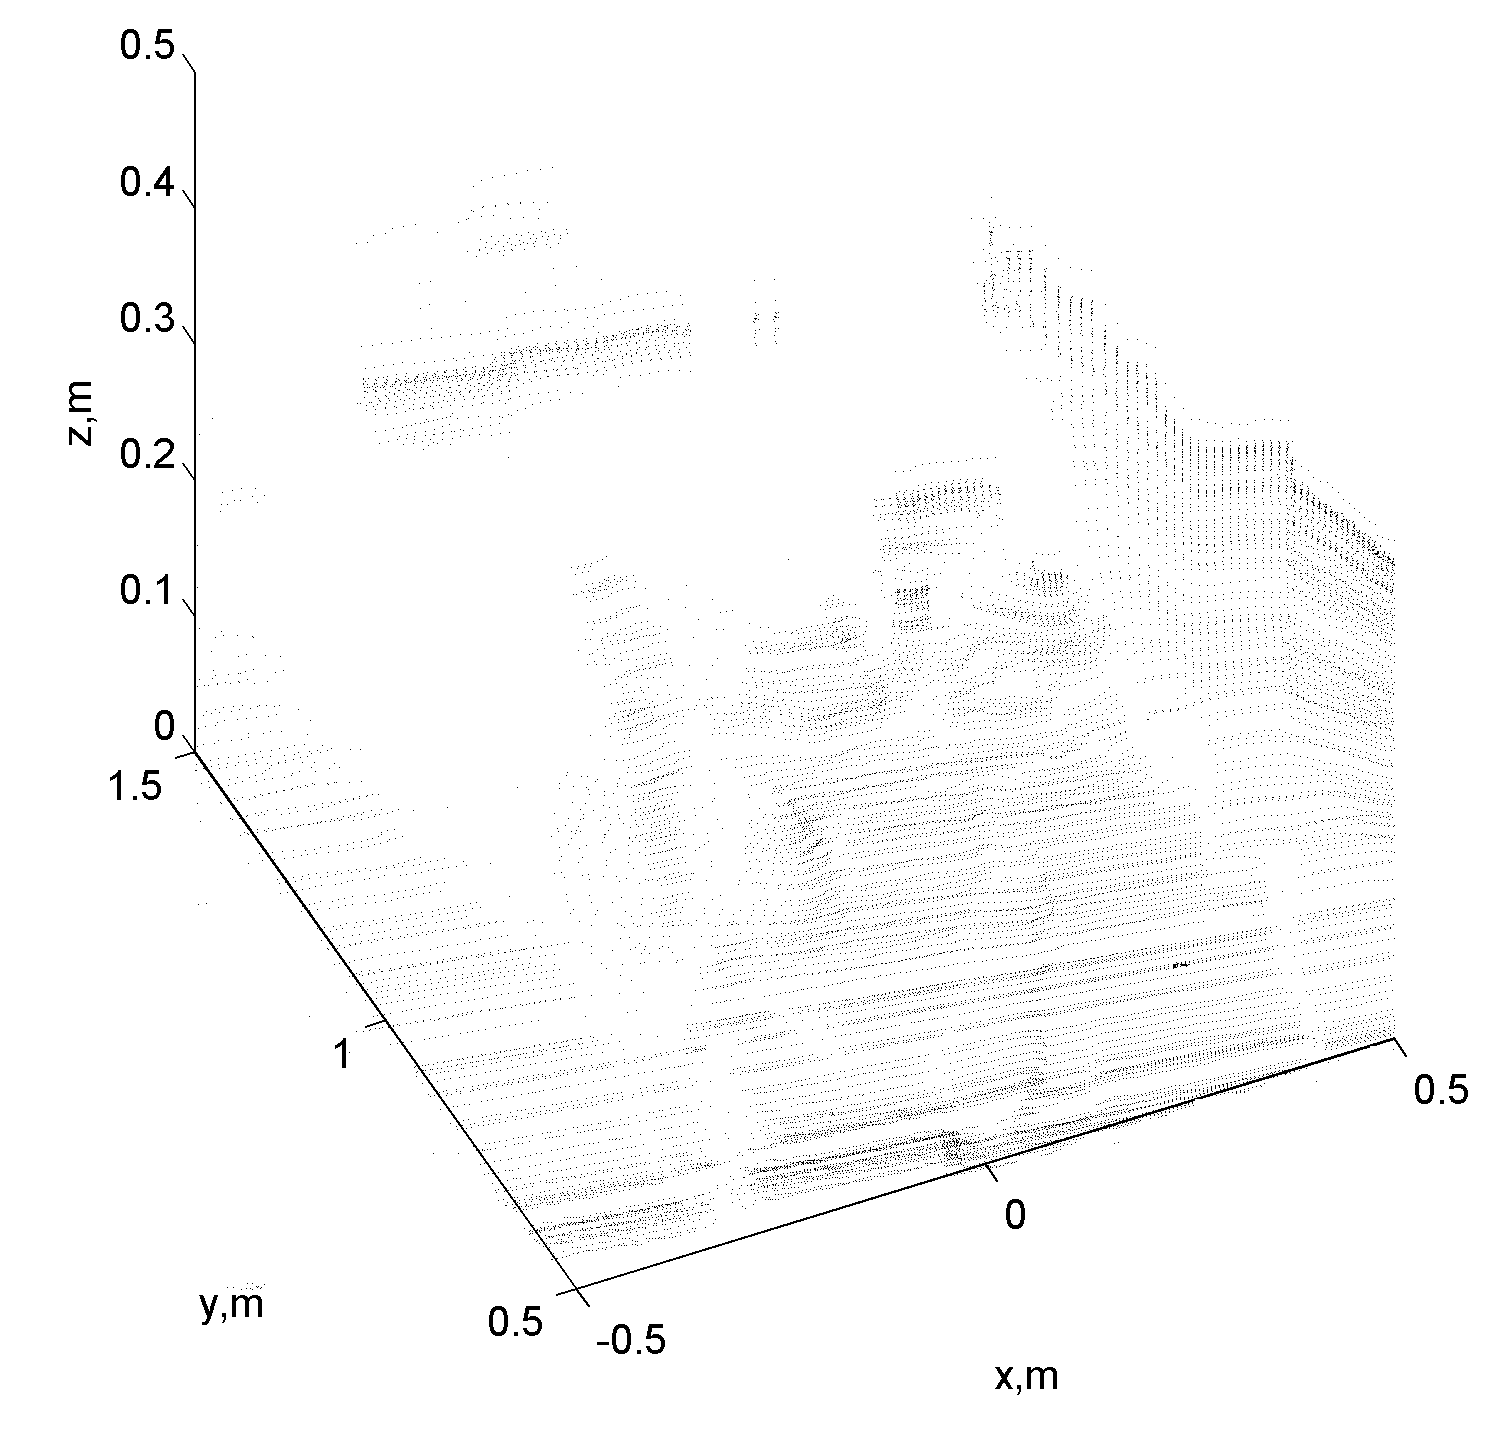
\includegraphics[width=\textwidth]{terrain_pcd3_cleaned.png}}
					\caption{Original 3D point-cloud of terrain patch.}
					\label{fig::pointcloud_terrain_patch}
				\end{figure}


		\subsection{Height-map Generation from 3D point cloud}
			
			3D point clouds can be transformed into height-map representations. These representations are convenient for use in planning as they can be converted into discrete cost-maps in a straightforward way. These height-maps are generated by populating the elements of a matrix  $M\in \Re^{n\times m}$ with the $z$ components of points which exist within discretized $w\times d$ region within the original 3D point cloud. The location and size of this regions would have to be determined with some auxiliary detection process which 1) determines that the area has high terrain variation, and 2) determines the bounding region where this patch of rough-terrain exists. We will call this patch a \emph{region of interest} (ROI). Once an ROI is determine, the 3D cloud containing only points from the ROI is isolated from $\bar{S}$ and divided into $(nm)$ sub-divisions, each of which covers a $(w/m) \times (d/n)$ area. Each (\Ith, \Jth) element of $M$, $m_{i,j}$, is then populated with the highest point (larger  $z$ component) within each  (\Ith, \Jth) subdivision. Depending on the density of the 3D point cloud, this process has the potential to produce relatively sparse height-map. To deal with this, a dilation and smoothing routine is used to complete the height-map conversion process. During dilation, each non-zero height element within the map is expanded into a region around the exiting element until. This process is performed until a semi-uniform map is produced with minimal gaps between non-zero height elements. Finally, a median filter is applied to the dilated height-map to produce smooth transitions between height elements.
				\begin{figure}[t!]
					\centering
					\fbox{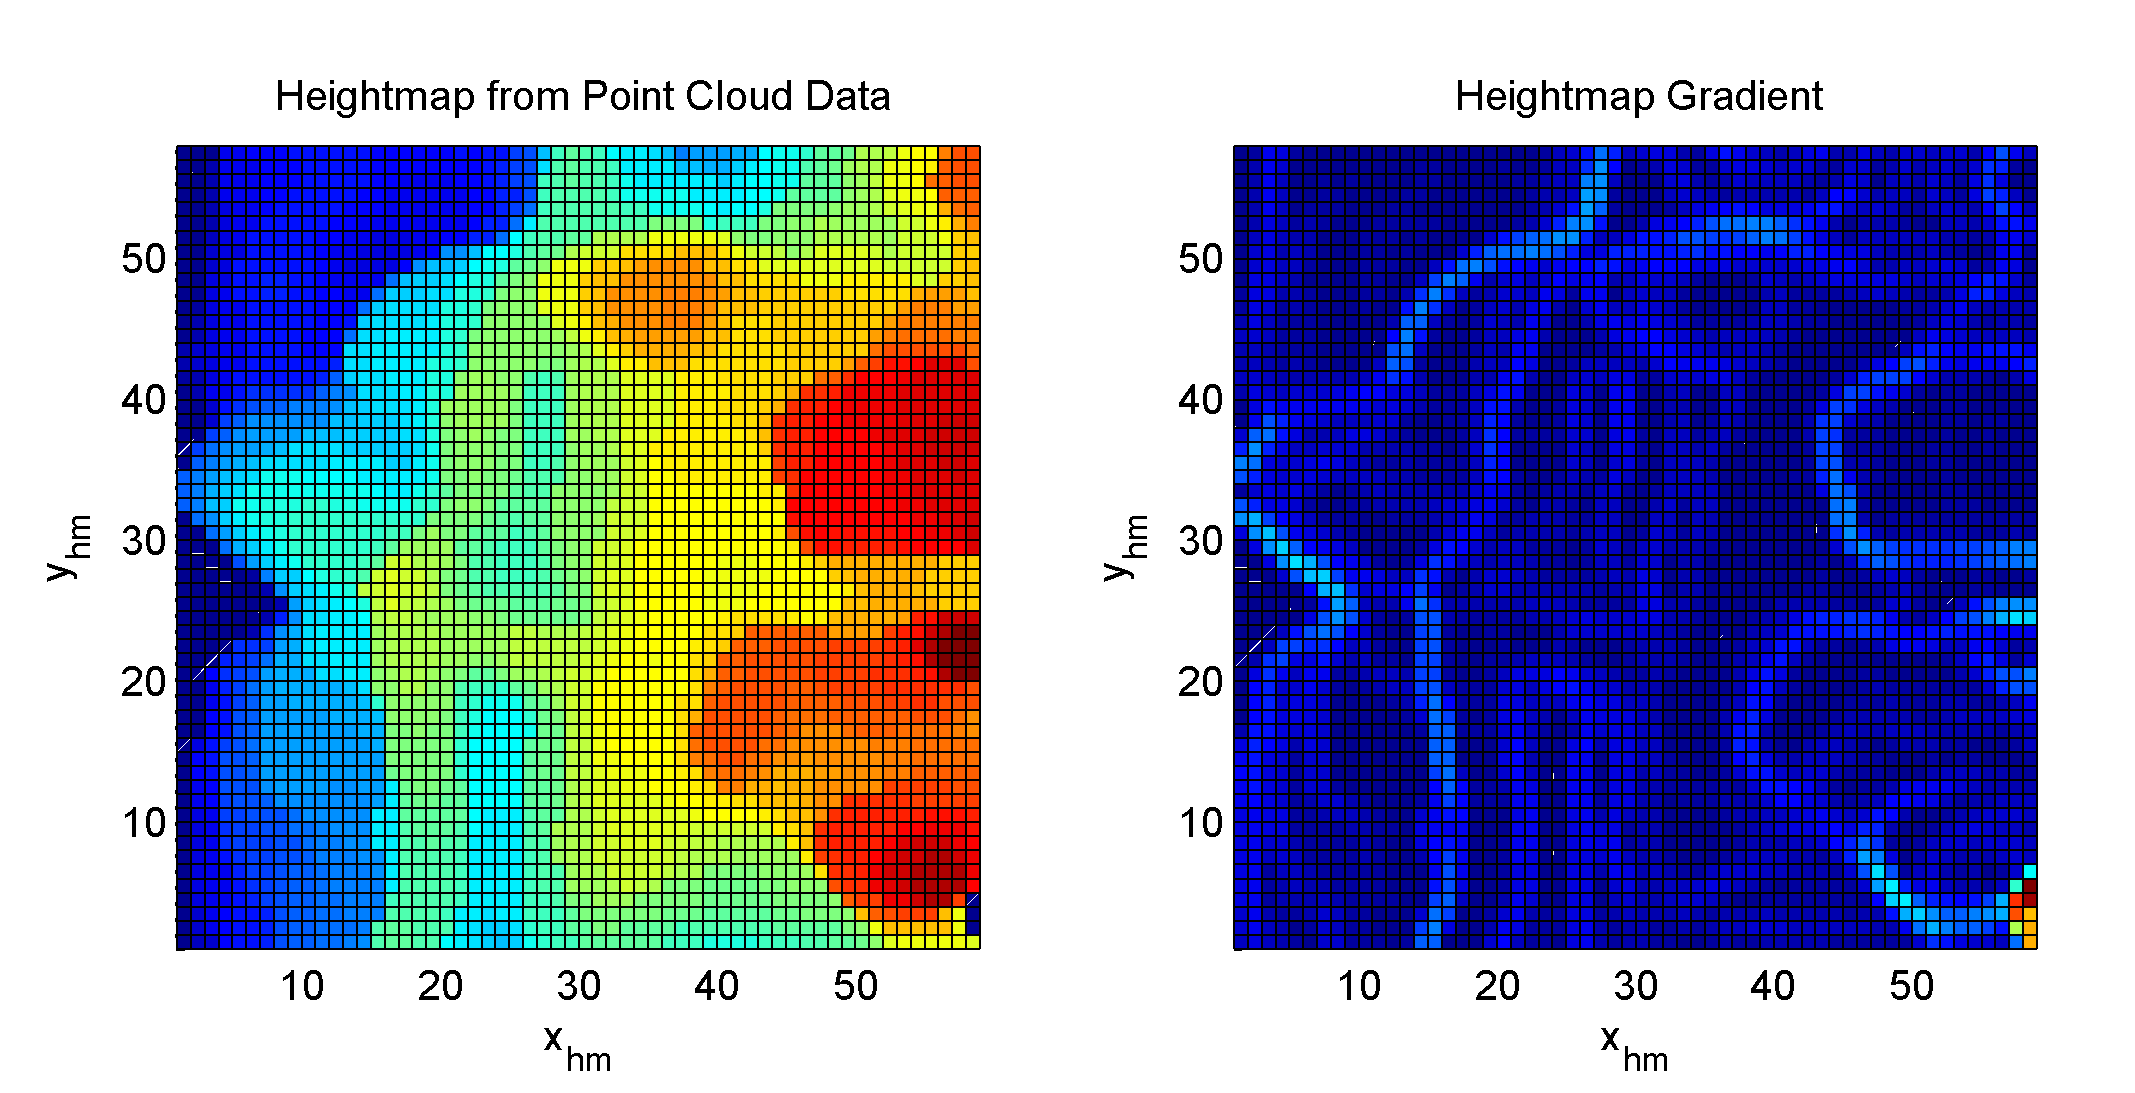
\includegraphics[width=\textwidth]{terrain_grad_crop.png}}
					\caption{Relative height-map \emph{(left)} and its corresponding gradient \emph{(right)}.}
					\label{fig::heightmap_terrain_patch}
				\end{figure}
				\begin{figure}[h!]
					\centering
					\fbox{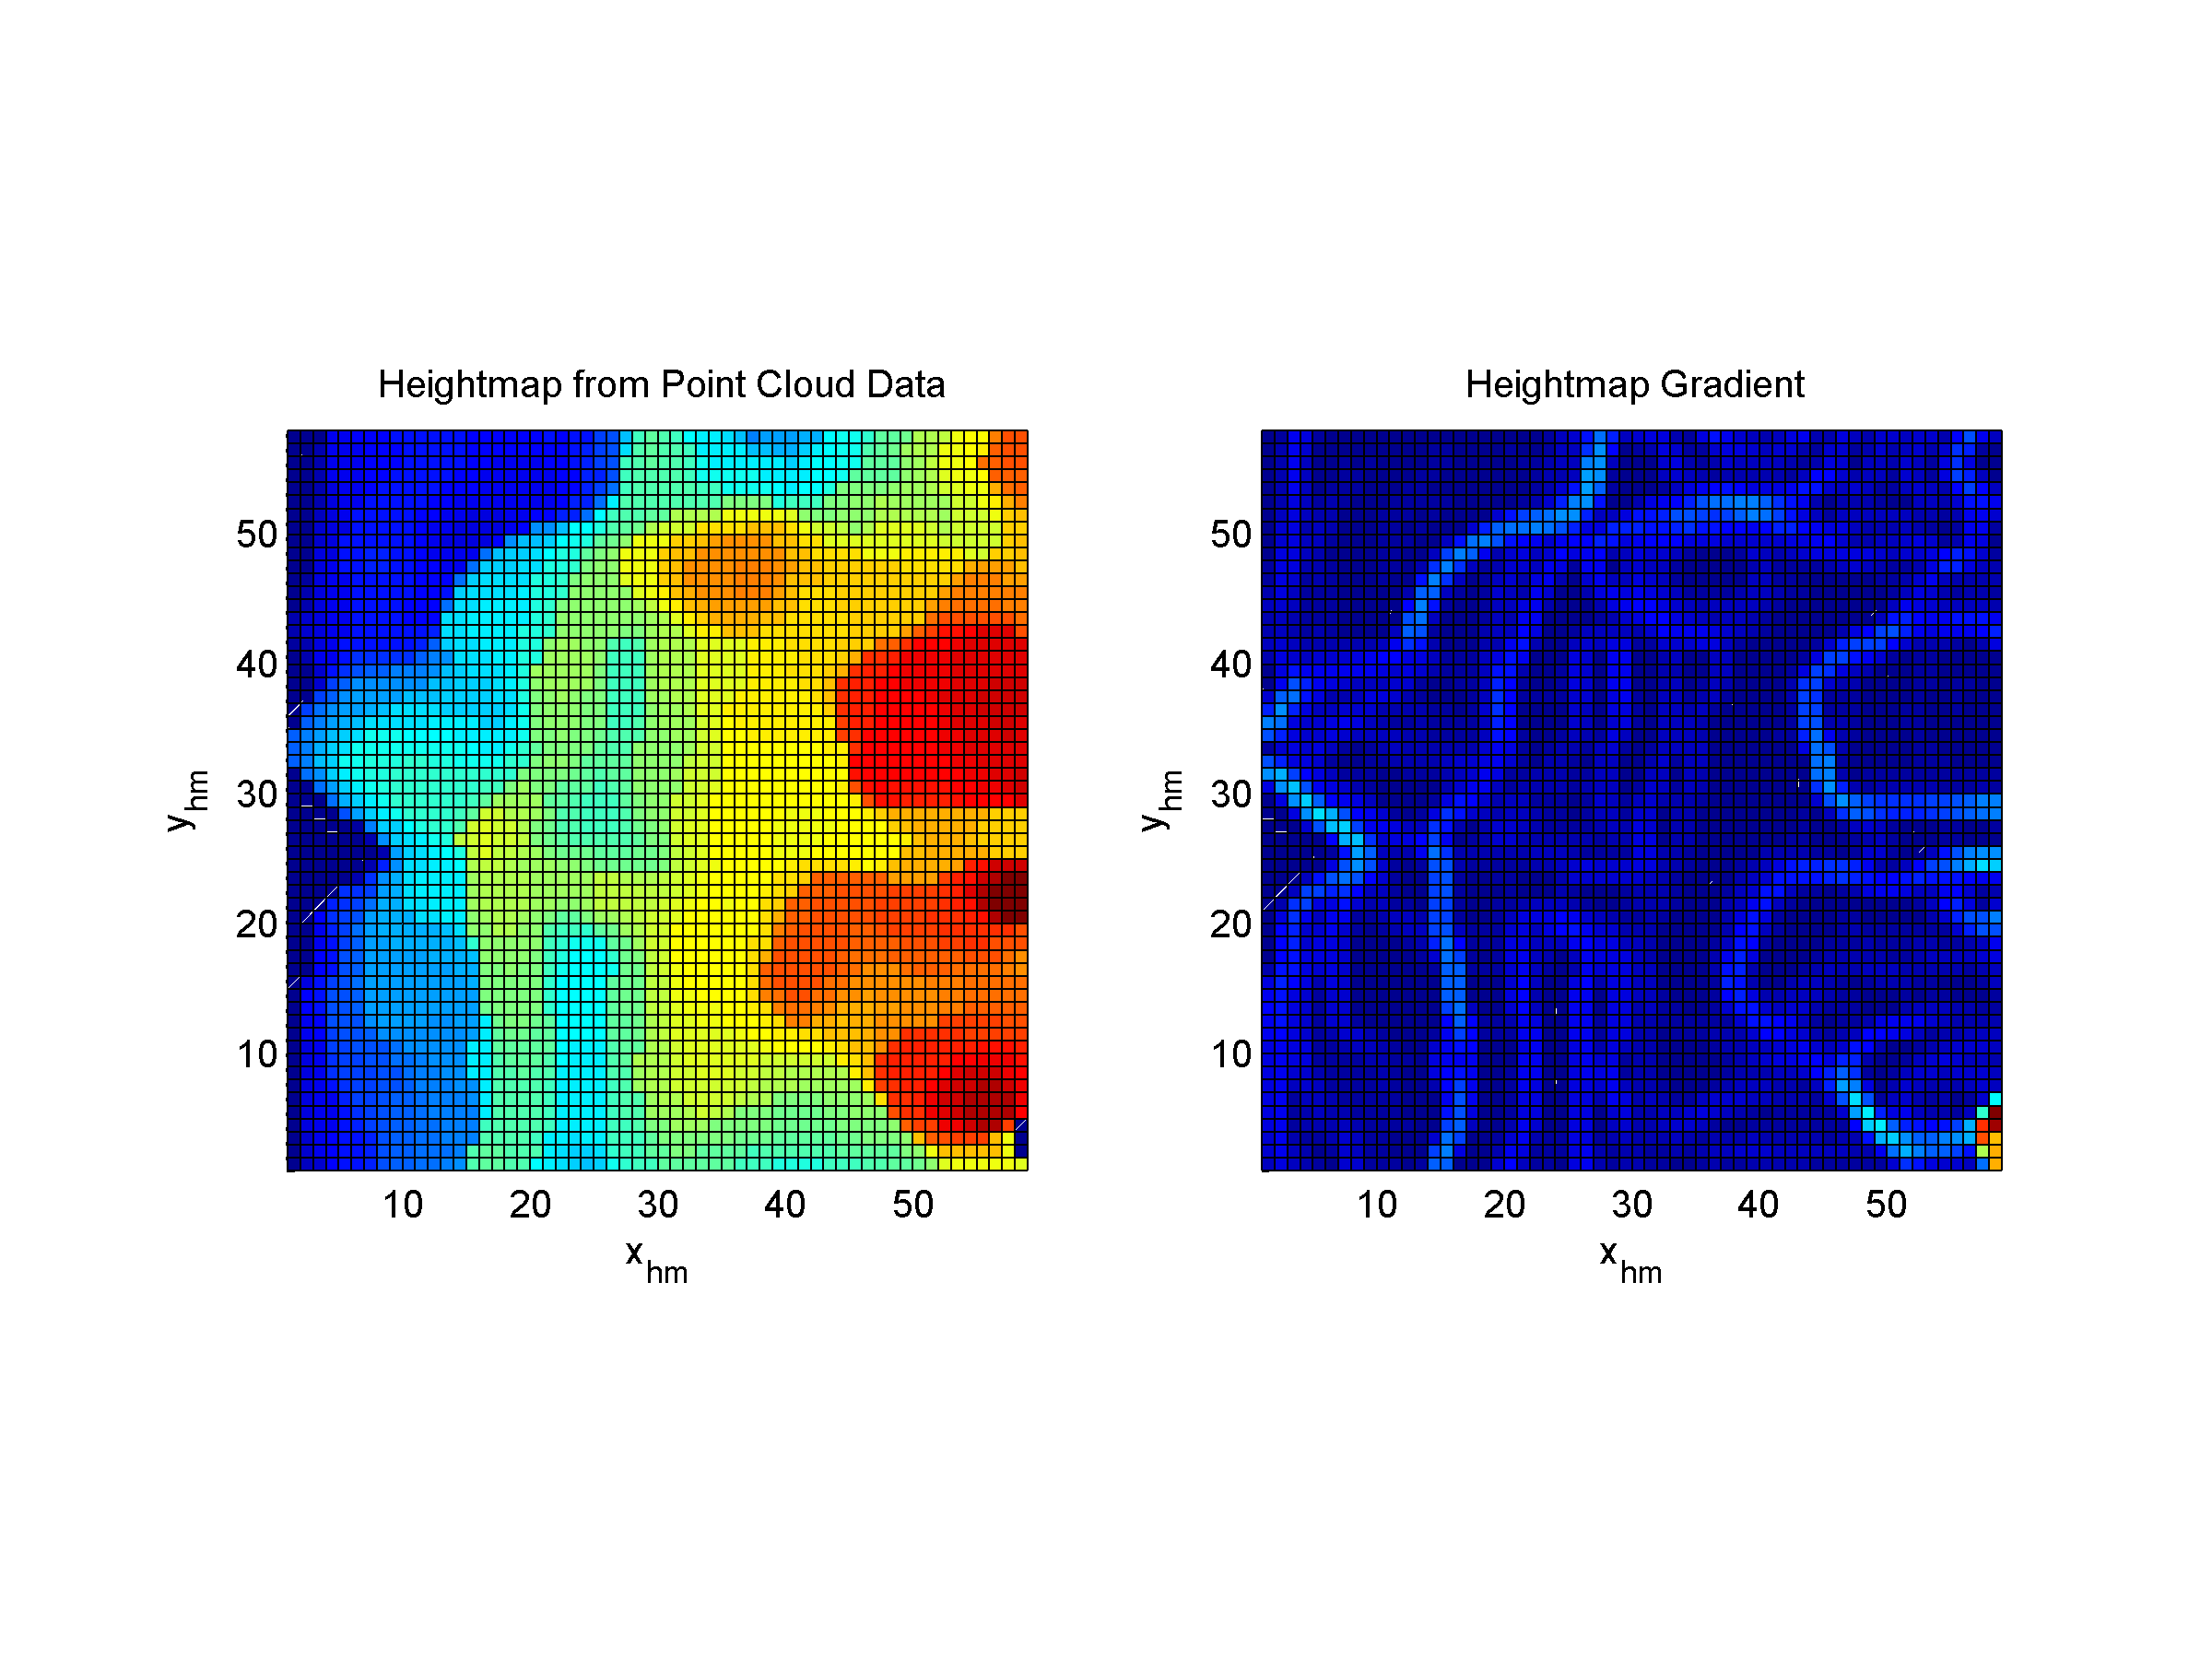
\includegraphics[width=\textwidth]{terrain_4545.png}}
					\caption{Height-map showing terrain variation in the $z_{hm}$ direction.}
					\label{fig::heightmap_terrain_patch_ortho}
				\end{figure}							
			The full 3D point cloud to height-map conversion is summarized in Algorithm \ref{alg::hmconvert}.
			\begin{algorithm}[!h]
				\begin{algorithmic}
					\State{\textbf{init} $M = \Theta, w, d, \bar{S}$}
					\State{$\bar{S}_{ROI} = \text{isolateROI}(\bar{S})$}
					\ForAll{$\bar{x}_{k}\in \bar{S}_{ROI}$}
						\State{$[i,j] = \text{getBestSubdivIndex}(\bar{x}_{k,1},\bar{x}_{k,2},w,d)$}
						\If{$\bar{x}_{k,3} > m_{i,j}$}
							\State{$m_{i,j} \leftarrow y_{k,2}$}
						\EndIf
					\EndFor
					\State{$M \leftarrow \text{dialateFeatures}(M)$}
					\State{$M \leftarrow \text{medianFilter}(M)$}
				\end{algorithmic}	
				\caption{3D ROI point cloud to height-map conversion.}
				\label{alg::hmconvert}
			\end{algorithm}

		\subsection{Surface Reconstruction}
			\begin{algorithm}[!h]
				\begin{algorithmic}
					\State{\textbf{init} $\bar{S},\bar{S}^{*},d,\vec{u}^{r},e,e_{max}$}
					\State{$\hat{S} = \text{voxelGridFilter}(\bar{S},d)$}
					\State{$\hat{S} \leftarrow \text{movingLeastSquaresFilter}(\hat{S})$}
					\State{$\hat{N} = \text{estimateNormals}(\hat{S})$}
					\ForAll{$\vec{n}_{i} \in N$}
						\State{$e = (\vec{u}^{r})^{T} \vec{n}_{i}$}
						\If{$e<e_{max}$}
							\State{ $\bar{S}^{*} \leftarrow \bar{S}^{*} \cup \bar{x}_{i}$ }
						\EndIf
					\EndFor
				\end{algorithmic}	
				\caption{Finding good places to step from a 3D point cloud.}
				\label{alg::goodspacestostep}
			\end{algorithm}


	%\subsection{Proposed Methods for determining the existence of Rough Terrain}

	%\subsection{Foot-placement planning}


